\section{Executive Summary Overview}
This notebook is the documentation of the FTC 4290 journey from right after the competition at World Championships up until the preparation for the San Antonio South Super Regional.\\

At World Championships, our team had the opportunity to observe best practices from the FTC teams at World Championship. We interacted with teams using technologies from programming Mecanum to Field Oriented Drive. We cheered for teams with fantastic strategy and superior autonomous programs. These teams motivated us to become a team that could compete on Edison or Franklin fields at World Championship.\\

We started work over the summer and organized subteams to work on build technologies, drive train strategies and autonomous coding. We assessed using LabView vs RobotC and made the decision to move to RobotC - introducing an open-source library that is easy for other teams to adapt into their own code.  Our goal was to put together a design, build it and provide the drivers with enough time to practice before qualifiers. We used a new design methodology and focused on rapid prototyping because we had very strong CAD and build skills with our seniors. We continued to support our outreach programs with our SMARTCamps and Robot demos. Our team was fortunate enough to have enough funding to buy a full field and game pieces. This enabled our drivers to practice and scrimmage with other FTC teams such as 5998 (Ultraviolet), 8399 (Austin Robotics Club), and 6299 (Viperbots QuadX).\\

To complement and facilitate communication and project management, we evaluated on-line methods including Trello to help improve our communications and project management skills. We decided after beta testing Trello, that we would use it for the 2014-2015 season.  This notebook was automatically generated from a Trello board using a software our team created - available open-source at \url{https://trello2latex.herokuapp.com}.\\ 

We have been proud of our performances at the 2 regional qualifiers that we participated in at West Ridge Middle School and at Connolly High School, both in Austin, TX.  We were undefeated, first seed in both qualifier and winning alliance captain in both.  At West Ridge Middle School, we were awarded Inspire 2nd place and at Connolly High School we were awarded Inspire winner.  At our last tournament, we won the PTC Design award as well as being part of the winning alliance.\\

We have enjoyed working together this season using the new design methodology. We have grown together as a team and look forward to the upcoming San Antonio Super Regional!\\

\newpage

\section{How to use this Notebook}
Notebook and communication are a key factor to success for any project. We had previously used a blog entry system and understood the pros and cons of keeping a notebook in that format.  This summer, the team started to evaluate and use new tools including Trello that is based on project management and tasks. It was encouraged by our industry mentors from National Instruments and IBM.  After our evaluation, we made the decision to proceed and have not regretted it.\\

Trello is a free project management tool that improves and enhance our team communications and documentation. We ran a parallel effort to use our regular notebook process and Trello until mid July. Our evaluation of Trello was favorable and we decided to use Trello for our project/tasks and were pleased with its success as a communication/documentation tool.  Our team members and our coach are all smartphone savvy and particularly liked being able to access the “notebook”, discuss, communicate and make decisions instantaneously.\\

Trello is able to time date stamp and log in all the thoughts/comments and work efforts of every member of our team. It can keep lists/tasks, host files, pictures, spreadsheets, links to other sites and tools, all in one easy to access place.  As such, our notebook moved from a date/time based organization to a project/tasked based effort.   We used the Trello2LaTeX tool, created by a member of our team, to create this notebook.\\

Our team members believe that Trello was integral to the success of our team by improving our project management and communication.  It has enhanced the chance of success by enabling 24x7 communication and documentation with pictures, links, videos posted right into the task card. We highly recommend Trello as a communication and documentation tool and our sister FRC team has chosen to use it for their upcoming season based on our success with this tool.\\

We have clarified through the FTC Q\&A that using Trello is an acceptable form for Notebook and used the Trello tools to print this notebook out. Below is the ruling:\\

\begin{figure}[H]
	\centering
	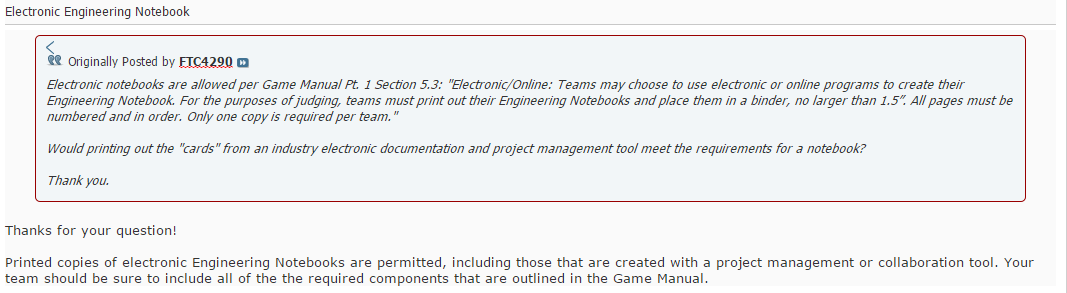
\includegraphics[width=\linewidth]{ruling}
	\caption[]{ruling.png}
	\label{fig:ruling}
\end{figure}

\clearpage
\newpage

\section{Our Trello board}
\begin{figure}[H]
	\centering
	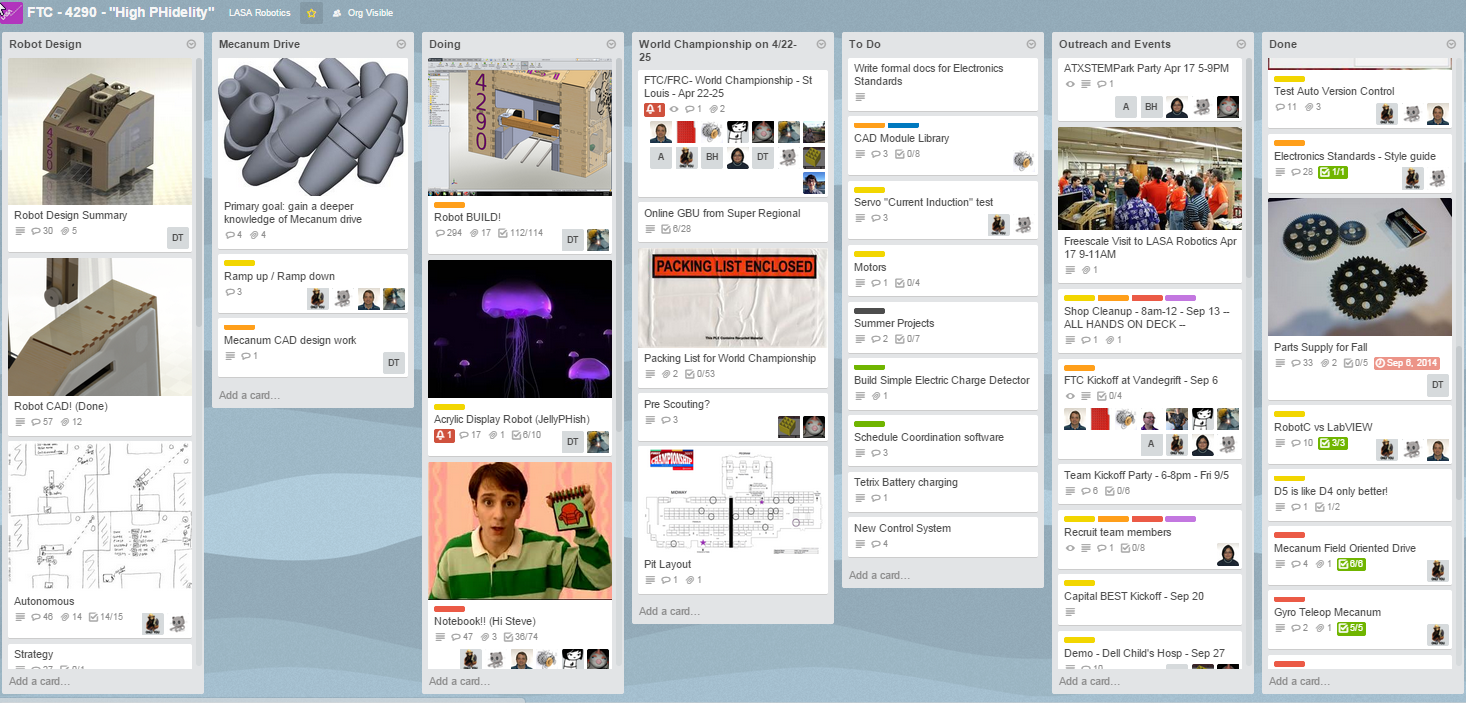
\includegraphics[width=\linewidth]{board}
	\caption[]{board.png}
	\label{fig:board}
\end{figure}
Above is an old version of our Trello board, as seen on Trello.com.
\clearpage
\newpage

\section{Team Overview}
\subsection{Team Mission Statement}
The Team mission is to inspire young people to be science and technology leaders, by engaging them in exciting mentor-guided, student-based programs that build science, technology engineering and math skills, that inspire innovation, and foster well-rounded life capabilities including self-confidence, communication, integrity and leadership.

\subsection{LASA Robotics Association Mission Statement}
The mission of the LASA Robotics Association is to support the LASA Robotics Team in developing and enhancing their skills and education to apply their knowledge, creativity, and intellect through a robotics competition format. The Association also serves as a conduit to facilitate community outreach, encourage entrepreneurial development, and provide community service opportunities.

\subsection{Team Origin}
The LASA Robotics team was formed in 1993 from students at LASA and LBJ High schools and is located in Austin, TX. LASA is the Magnet school in the Austin Independent School District, housed on the same campus as the 98\% minority composition LBJ High School. This “dual school, one voice” format allows the LASA Robotics Team to be very diversified in both student makeup and educational backgrounds.   Originally formed to compete in the BEST Robotics Competition, MATE, and TCEA Robotics, the team now primarily competes in the FIRST Tech Challenge (FTC) and FIRST Robotics Competition (FRC).  We use FIRST competitions to hone in our critical thinking; improve our engineering skills in a fun environment, celebrating teamwork while competing.\\

LASA Robotics has a rich history with FIRST Robotics spanning 15 years. We serve as a breeding ground for future inventors and engineers, but we also give other motivated students the opportunity to experience a well-rounded STEM education. We have over 400 Alumni, many have studied in the engineering and science fields and are successful in industry or research fields. Appendix A lists our FIRST Awards and Achievements.   The coach of the team has always been Mr. Anthony Bertucci.\\

\subsection{Team Organization}
The LASA Robotics Team is comprised of FRC 418 and FTC 4290 and FTC 5998.  In 2014-2015, we have 75 members that are registered to participate with 27 Freshman on the team.  Every year, the team elects their leaders to help guide the team.  The FTC team roles this year are Drivers/Operators, Build, Programming, Notebook, Artistic Design, Scouting and Presentation.  Students in each role could and did participate in multiple groups.  Besides the official team leadership, we encourage team members to form impromptu groups to accomplish specific tasks supporting robot demos, repairs and other smaller projects that need to get done.\\

As we are a magnet high school with students from all over Austin, many of our students are dependent upon the late school buses to get them home from after school activities.  This requires that students meet after school from 3:45PM to 6PM on Monday - Thursdays.  Many of our students don’t get home until past 7PM on the weekdays that the team meets.  Our meeting and work schedule also dictate that we have mentors that can support this schedule, limiting the industry employed mentors that have the flexibility to work with the team.   

\begin{figure}[H]
	\centering
	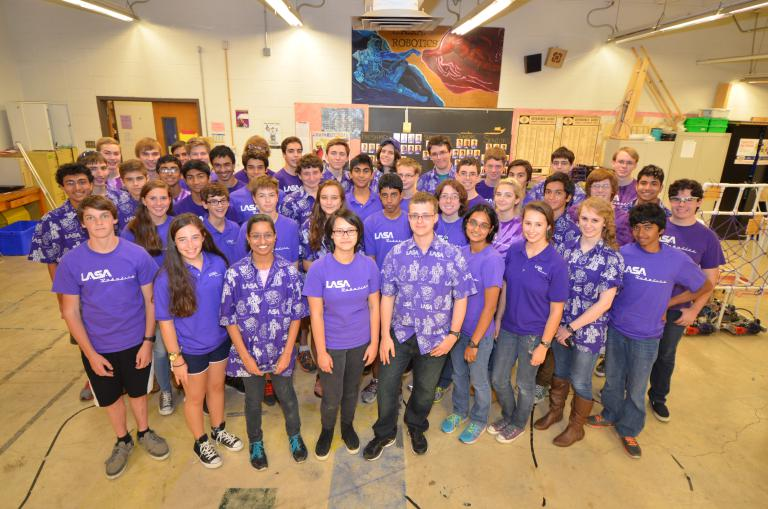
\includegraphics[width=\linewidth]{teamorg}
	\caption[]{Our team, 2014-2015}
	\label{fig:team}
\end{figure}

\subsection{Current Team Status}
There are currently 75 members on the team, a 60+\% increase from 3 years ago. The team has overcome many challenges associated with rapid growth, such as building a student leadership and becoming better organized to more efficiently manage the students on our team while still providing all team members with a rewarding, interesting, and educational experience without exceeding our budget. Almost one third of the students are on the free and reduced lunch program and require scholarships for individual expenses which include travel, snacks and team shirt costs. LASA Robotics does not limit the size of the team nor require applications to join, keeping our financial goals and needs a moving target. 

\clearpage
\newpage

\subsection{Team Biographies}
\begin{wrapfigure}[7]{l}{1in}
	\centering
	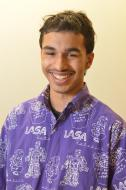
\includegraphics[height=1in]{ehsan}
\end{wrapfigure}
\subsubsection{Ehsan Asdar - Junior - Programmer} 
I like that we all are working together towards a challenging goal. The way the FIRST competitions are built require the team to have structure and organization, get things done in a timely manner and collaborate. Since I am on programming, I especially enjoy the software aspect which is basically taking a giant oddly-shaped piece of metal and making it do something.

\begin{wrapfigure}[7]{l}{1in}
	\centering
	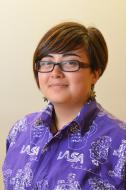
\includegraphics[height=1in]{julia}
\end{wrapfigure}
\subsubsection{Julia Cocco - Junior - Project Coordinator / Notebook}
Chemistry is the class I enjoy most. I find chemistry to be both fascinating and fun, because the rules are simple once you've learned them (and there are very few exceptions). The logic behind what we do makes sense to me, and I can rationalize through most problems with relative ease.

\begin{wrapfigure}[7]{l}{1in}
	\centering
	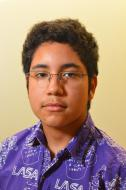
\includegraphics[height=1in]{izzy}
\end{wrapfigure}
\subsubsection{Ismael Flores - Senior - Design / Alternate Driver} 
- Physics, for perspective\\
- English, for enlightenment\\
- Robotics, for application

\begin{wrapfigure}[7]{l}{1in}
	\centering
	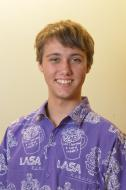
\includegraphics[height=1in]{blake}
\end{wrapfigure}
\subsubsection{Blake Hance - Junior - Driver} 
The people on the team are my favorite part.  I have always had a knack for understanding it, and I enjoy learning it. I also plan on going into either chemistry or biotechnology and do research.

\begin{wrapfigure}[7]{l}{1in}
	\centering
	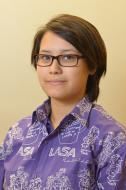
\includegraphics[height=1in]{kyla}
\end{wrapfigure}
\subsubsection{Kyla Hayworth - Sophomore - Operator} 
Well, robots are pretty cool. I would like to go into something like electrical engineering.  I'm planning on going to MIT and finding out what I want to do from there. \\

\begin{wrapfigure}[7]{l}{1in}
	\centering
	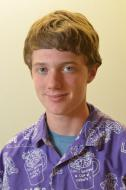
\includegraphics[height=1in]{jackson}
\end{wrapfigure}
\subsubsection{Jackson Hughes - Junior - Driver} 
The people on the team are my favorite part.  I have always had a knack for understanding it, and I enjoy learning it. I also plan on going into either chemistry or biotechnology and do research.

\begin{wrapfigure}[7]{l}{1in}
	\centering
	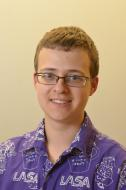
\includegraphics[height=1in]{arthur}
\end{wrapfigure}
\subsubsection{Arthur Pachachura - Junior - Programmer /  Marketing / Notebook} 
I get to do all sorts of weird stuff, help lead a team's programming department (considering there are only really two of us in FTC), and more weird and random stuff when no one is looking. ;)

\begin{wrapfigure}[7]{l}{1in}
	\centering
	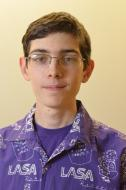
\includegraphics[height=1in]{daniel}
\end{wrapfigure}
\subsubsection{Daniel Teal - Senior - Design / Build} 
I really enjoy making things work.  My favorite subject is Math. Any kind. Physics included. It all makes so much sense!  My hobby is rapid, precise manufacturing of things and ideas and tools to make them; recycling, rebuilding, and 3D printing included. Legos are fun, too.

\begin{wrapfigure}[7]{l}{1in}
	\centering
	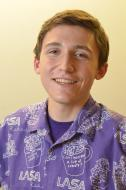
\includegraphics[height=1in]{marek}
\end{wrapfigure}
\subsubsection{Marek Travnikar - Senior - Design / Build} 
Robotics - really it actually takes up my entire free time. Other than robotics, my main hobby would be home made weaponry, such has my arsenal of trebuchets, potato cannons, actual cannons, and fire arms built under an FFL. I plan to dual major in Mechanical and Electrical Engineering, possibly minoring in Computer Science (there is a trend here). 

\clearpage
\newpage

\section{Outreach Overview}
The LASA Robotics Team is committed to outreach.  We participate in various demos and outreach programs throughout Central Austin.  This year, we have been very active and kicked off the season with  3 of our team members volunteering at the World Championships on the Franklin and Curie Fields and two of our mentors volunteering to judge the FTC competition at World Championships.  We continued our support of FLL and held SMARTCamps and our team member, Arthur created an FLL program to train rookie coaches.\\

Our goal is to expand access to robotics and STEM in our community. We are working with the City of Austin, industry and Austin Community College to create a permanent Robotics/STEM space in Austin – an intellectual rec center. We’re working with FIRST president Don Bossi to engage industry leaders and state legislators to recognize STEM and robotics as a Texas UIL approved extracurricular academic activity, which will impact more than 1200 districts with more than 5 million students statewide.\\

Our LASA Robotics SMART Camps introduce FLL to Title I and other schools, inspiring them to start teams. Through this camp, we recruited enough interest at the Texas School for the Blind to start the “DOT BOTs”, the first Blind FLL team in the world. Using our fabrication skills, we built over 25 regulation FLL Tables for area teams and competitions. This year, a new effort supports 10 rookie FLL Coaches, training them in programming and giving them guidance in judging and competition logistics.\\

At FLL-focused events and competitions, we provide FTC demos to encourage students to consider progressing to the FTC program. At our family outreach events, including Formula 1, Fun Fest, MakerFaire, Dell Family Day, Freescale events and others,, we have demonstrated  FTC and FRC demos to over 46K people in the past 2 years, exciting students about STEM and encouraging participation in FIRST. We host an annual gathering inviting all area FTC and FRC teams to join and build community.\\

At FLL competitions, we serve as referees, judges and logistical support. At FTC competitions, we are well-known for being a “go-to” resource and problem solvers; our FTC members even help other teams in the challenge box. For FTC and FRC competitions, we give out peer awards to encourage other teams. This season, FTC 7079 and their school superintendent recognized LASA Robotics as the Gracious Professional team they hope to emulate. Our new STEM Park provides free practice space for all teams.\\

Below is a table with the dates and event supported by our outreach programs:

\begin{figure}[H]
	\centering
	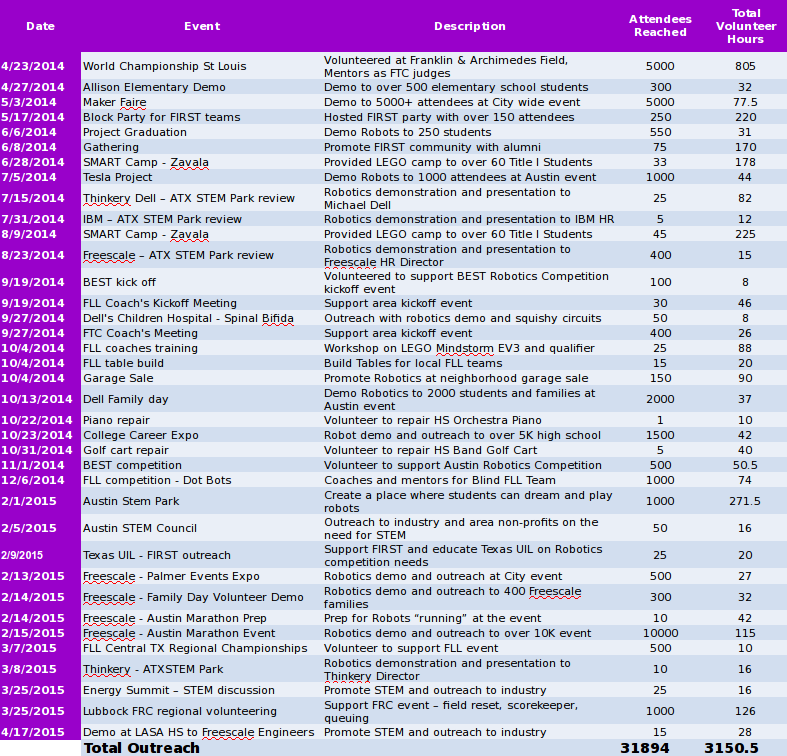
\includegraphics[height=0.6\linewidth]{outreach}
	\caption[]{LASA Robotics Outreach Activity (Through Feb. 2015)}
	\label{fig:reach}
\end{figure}

To date, LASA Robotics has logged over {\bf 2107 hours} and reached over {\bf 18,300 people} in our outreach and volunteer events.

\section{Business Plan}
\subsection{LASA Robotics Association}
The LASA Robotics Association is the key to the financial sustainability of the LASA Robotics Team.  The Association is comprised of parents and supporters of the LASA Robotics Team.   We have a president, vice-president, treasurer, secretary and executive director.  In addition, we have 3 parent representatives that participate in decisions.  We hold monthly meetings that are attended by the team coach, team mentors and a student representative. We abide by a set of by-laws that govern the Association’s operations.\\

To help with managing the team operations, we plan an annual budget. We have a documented financial process for team expenditures. The Association requires expenses be authorized through the budget process and any expenses exceeding the budgeted amount must be approved by the board. The treasurer presents a monthly report and only 4 people have check signing authorization at any time. In 2012, an independent bookkeeper completed an audit of our finances and no discrepancies were identified. For the 2014-2015 season, our budget is \$45,750.  See attached budget at the end of the Business Plan Section.\\

To help raise funds, we rely on grants, solicitation of funds from our family, friends and local businesses (ASK) and other fundraisers including paid Robotics Camps (SMART Camps), building FLL tables and selling handmade robotics jewelry.  To help with grants, we have a documented grant process where we seek and identify sponsors to help support the team. In the past 6 years, we have not had any issues with recruiting parents to join the LASA Robotics Association.

\subsection{Fundraising and Sustainability}
For the upcoming season, we are putting into place several actions to improve our financial positions.

\subsubsection{ASK}
Our ASK fundraiser has traditionally raised between \$5-\$7K with about 60\% participation.  Our team is now requiring that all students participate in the ASK fundraiser as a condition of travel to increase the participation rate and the total amount raised.  

\begin{figure}[H]
	\centering
	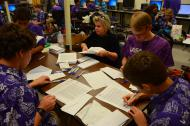
\includegraphics[height=0.3\linewidth]{ask}
	\caption[]{ASK Fundraiser}
	\label{fig:ask}
\end{figure}

\subsubsection{Grants}
We are actively recruiting parents to specifically help write grants.  Instead of working with one or two parents and training them to do this, we are working to put together a boilerplate for grant responses so that more parents can quickly get on board and help apply for grants.  Our grant strategy outlines a process where we focus our applications to companies that are already supporting FIRST Robotics.  This year, we were successful at applying for and receiving our first grant from Intuitive Surgical Incorporated, receiving \$1K for our FRC 418 team.\\

We strive to maintain long-term, mutually beneficial relationships with all of our sponsors. Some of our sponsors, such as 3M, have supported consistently for many seasons. At the end of each season, we hold a sponsor’s recognition event where we invite the team sponsors to come and see our team in action. In addition, we present our key sponsors with an engraved plaque as a token of our thanks. We also recognize those family, friends and businesses who respond to our ASK fundraisers by sending them a personalized thank you note along with a picture of the team in action.  
Our sponsors are shown in the chart above.

\begin{figure}[H]
	\centering
	
\includegraphics[height=0.3\linewidth]{sponsors}
	\caption[]{Our sponsors}
	\label{fig:sponsors}
\end{figure}

\subsubsection{Our Partnerships}
Many long-term sponsors continue to support us with grants: 3M, NI, Time Warner, Texas Workforce Comm, BAE and Smallworks. Two new sponsors joined last year: Intuitive Surgical and Altera. This year, we added Freescale and DELL. New partnerships with Austin Community College and UT Austin provide spaces for a STEM/Robotics Park and our SMART Camps. Other sponsors include Dassault Systems, IBM, Sherwin Williams, Home Depot, Whataburger, Metals4U, Main Street Hub and Hill Country Tactical.\\

We have worked hard to retain and recruit sponsors by developing and executing a grant strategy, doubling our grants to over \$15K in the past 2 years. We send all donors season updates about the team and recognize key sponsors with handmade wood plaques. Team members took robots to a marathon sponsored by our sponsor Freescale. The ATX STEM Park is a new partnership, involving shared community building, outreach and media coverage with Freescale, 3M, Austin Community College and City of Austin.\\

\begin{figure}[H]
	\centering
	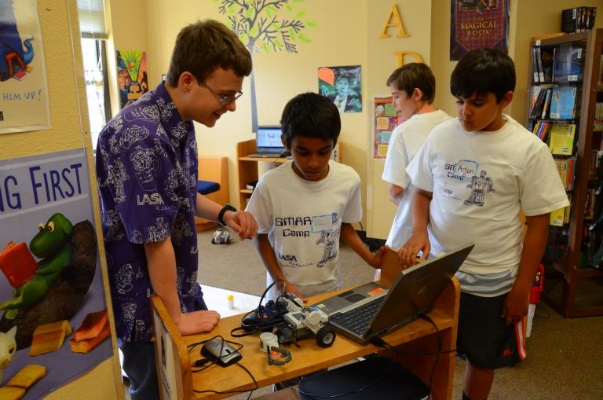
\includegraphics[height=0.3\linewidth]{smart2}
	\caption[]{SMART Camps}
	\label{fig:smart2}
\end{figure}

\subsubsection{SMART Camps}
LASA Robotics created the SMART Camp (Science, Math and Robotics, Technology) to help spread interest in Robotics and STEM. Using the LEGO Mindstorms kits, we provide a challenge for students to build, program and have fun with Robots. Our students serve as the mentor for these students ages 8-13. We provide a SMART Camp T-shirt and a healthy snack to all participants. These camps have served over 1000 students in the Austin area in the past 6 years, some of whom are currently members of the LASA Robotics Team. We use these SMART Camps as both for outreach and as a team fundraiser.   The outreach camps serve Title I schools and the Texas School for the Blind and Visually Impaired. We apply for Grants with companies such as 3M and Time Warner to provide these camps free of charge to students. For a fundraiser, we charge students \$40-\$50 for the beginner and advanced. The team continues to support and provide SMART Robotics Camps to help inspire younger students from all social-economic areas in Austin. The team and the mentors invite prospective sponsors, students and parents to come visit the robots at school and at our outreach and competition events to get a better understanding of the team and the FIRST program. The team mentors working with Texas School for the Blind and Visually Impaired (TSBVI) coach of the “DOT BOTS” FLL team to submit a paper to the national organization, the Association for the Education and Rehabilitation of the Blind and Visually Impaired, discussing how blind students can successfully participate in the FLL programs.\\

To help enable all students to participate in FIRST Robotics, the LASA Robotics Association has put together a fundraising plan that sets aside support for scholarships. These scholarships are available to students on the team to help with related team expenses. Last year, over \$2000 was given to help support team travel. This year, we are allocating \$3850 to support scholarships.

\clearpage
\newpage

\subsection{Risk Analysis}
\subsubsection{Team Strengths}
\begin{itemize}
	\item Commitment from our coach and mentors
	\item Our student body possess strong interest in STEM
	\item Educated and engaged parents
	\item Strong and long term relationships with key sponsors
	\item Strong FLL robotics program in feeder schools
	\item Student lead team
\end{itemize}

\subsubsection{Team Weaknesses}
\begin{itemize}
	\item Need more industry mentors to support team in electronics and public relations
	\item Our coach is within retirement age
	\item School and District provide limited support
\end{itemize}

\subsubsection{Team Opportunities}
\begin{itemize}
	\item FIRST is gaining momentum
	\item Industry Sponsors are becoming more committed to STEM
	\item City and State are interested in making Texas a knowledge economy
\end{itemize}

\subsubsection{Team Threats}
\begin{itemize}
	\item Expense of participation in FRC program
	\item Loss of Industry sponsorships if the economy stalls/declines 
	\item Increase in travel costs to competitions
\end{itemize}

\subsection{Risk Mitigation Plan}
Team must recruit more industry mentors from:
\begin{itemize}
	\item growing pool of team parents
	\item from our industry sponsor companies
\end{itemize}

Team must work with the school:
\begin{itemize}
	\item to identify, recruit and train potential replacement coaches.
\end{itemize}

We must improve public relations by:
\begin{itemize}
	\item highlighting the benefits of having a FIRST Robotics team
	\item lobbying to increase the support provided by the school administration
\end{itemize}

We must increase our fundraising:
\begin{itemize}
	\item because of possible increases in FRC program costs
	\item to help supplement student travel costs to competitions and team scholarships
\end{itemize}

We must increase and diversify our sponsorship:
\begin{itemize}
	\item to mitigate adverse economic effects to one industry sector 
\end{itemize}

\newpage

\section{Budget}
On the following pages is the team's budget for the 2014-2015 year.

\begin{figure}[H]
	\centering
	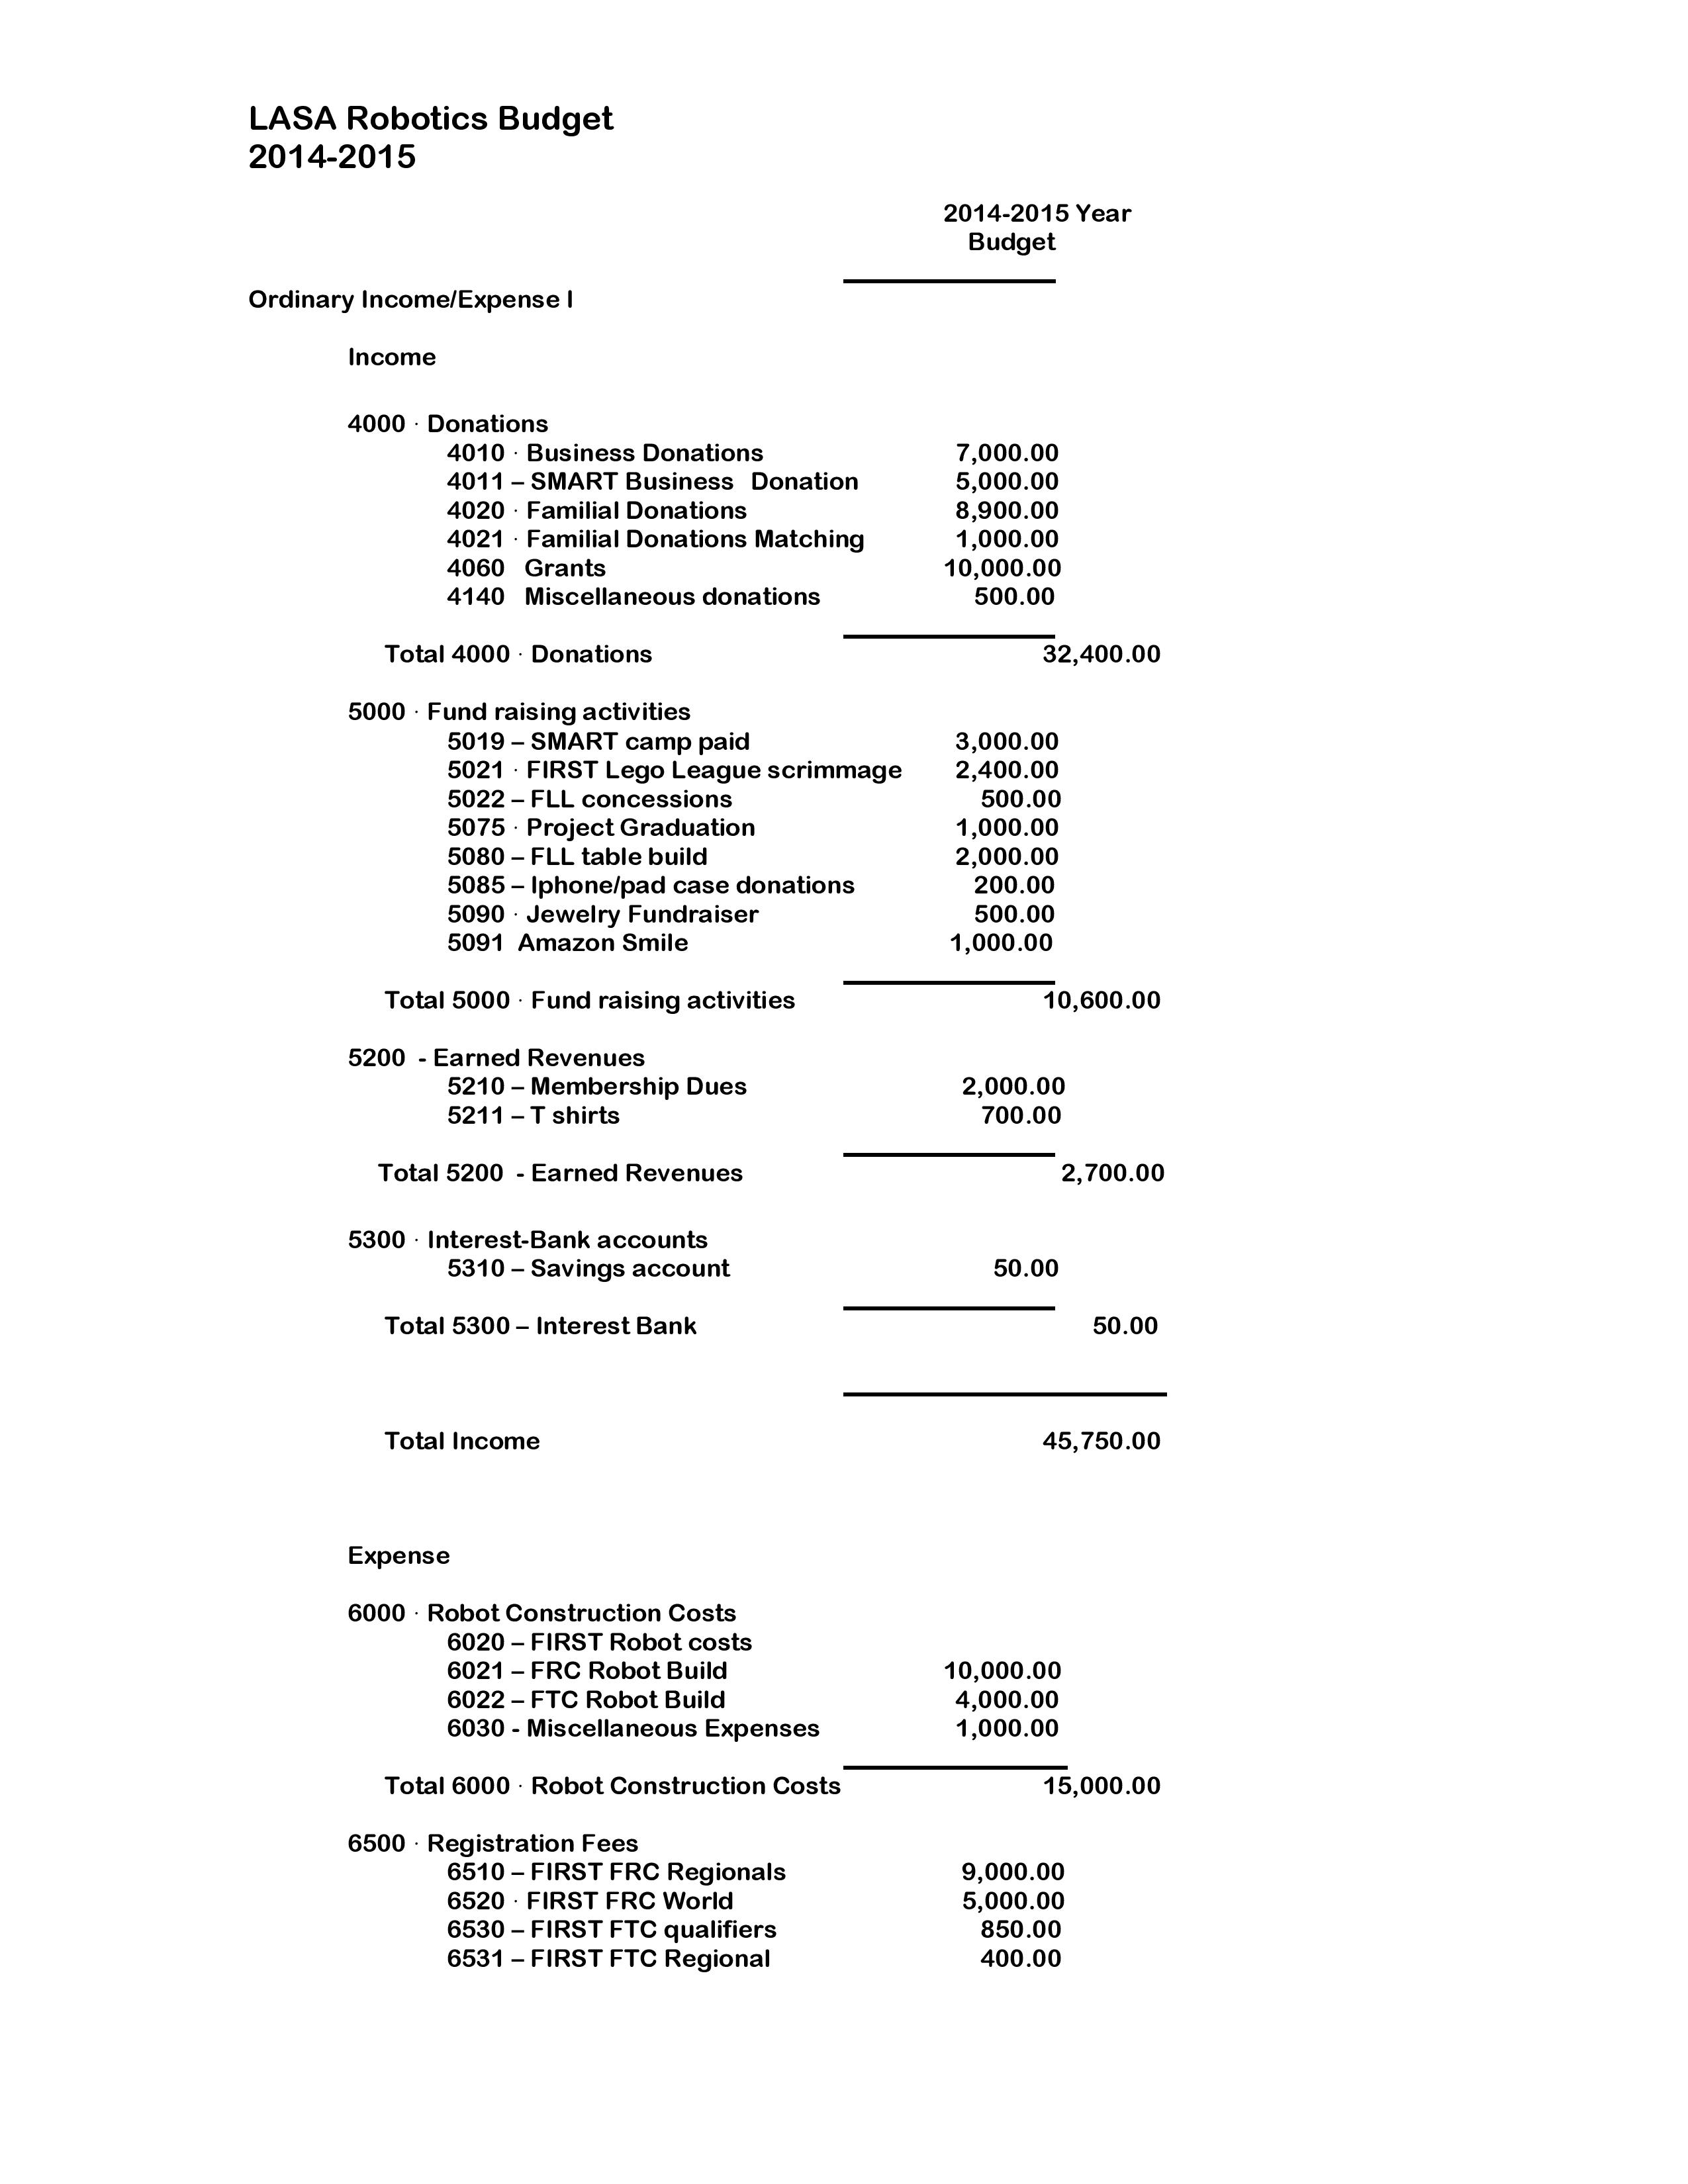
\includegraphics[width=0.9\linewidth]{budget}
\end{figure}
\begin{figure}[H]
	\centering
	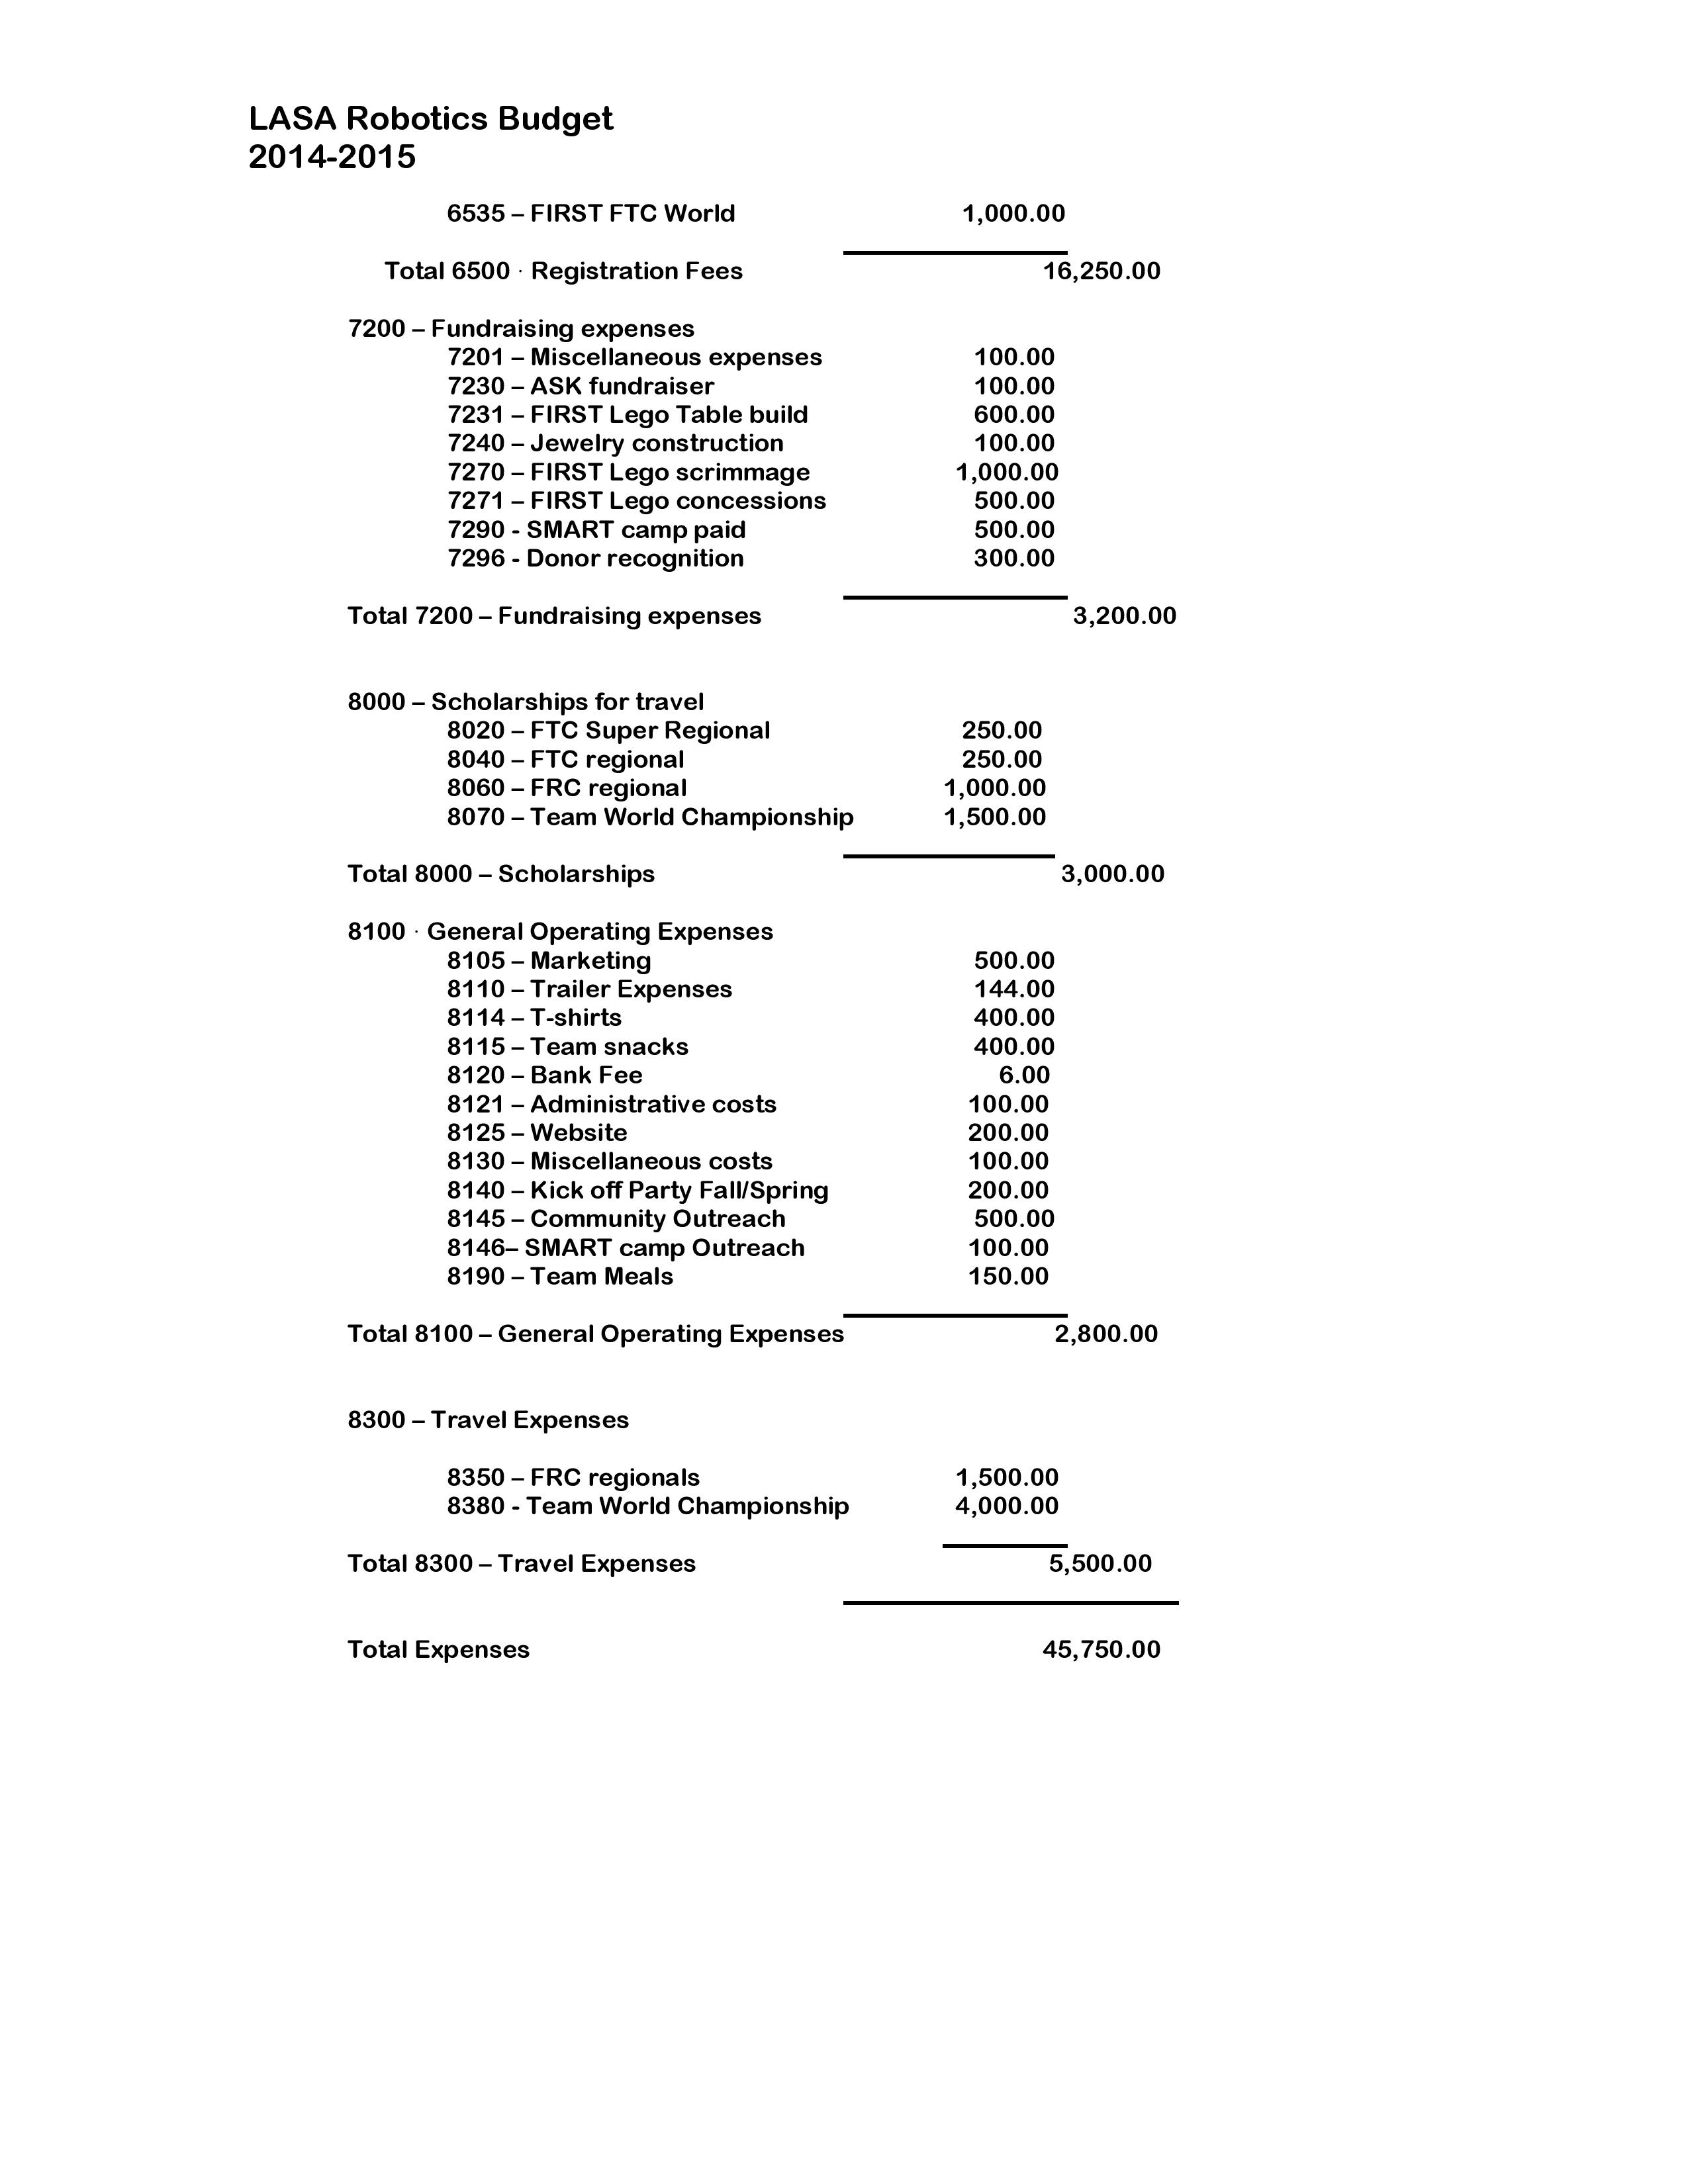
\includegraphics[width=0.9\linewidth]{budget2}
\end{figure}
\begin{figure}[H]
	\centering
	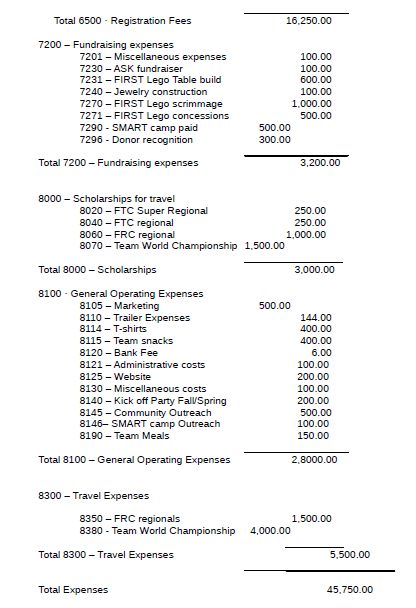
\includegraphics[width=0.9\linewidth]{budget3}
\end{figure}

\newpage
\clearpage
\newpage
\clearpage
\newpage
\color{black}